\chapter{Pin Control Attack}
\label{chap:attack}

Before describing Pin Control Attack, a deeper analysis of the architecture of the target system is needed.
Note that, although this paper is focused on PLCs, the architecture described in the next section is still valid for almost any embedded system.
After having a proper knowledge of the underlying architecture, we can go deep into the description of the design of Pin Control Attack.
We consider the idea behind the attack, showing how it is able to evade the currently available detection mechanisms.
Next, we go further and describe some implementations of the attack, extending its applicability to a real Programmable Logic Controller.
Based on our architecture analysis and our tests, we can finally demonstrate that the attack is actually viable on real PLCs, even on a higher abstraction level.


\section{Embedded architecture}
\label{sec:embed_arch}

As briefly reported into \mychap{chap:intro}, PLCs use I/O interfaces to communicate with sensors and actuators, and in general with any external device.
Digging into their architecture, we know that PLCs are usually based on a so called System on Chip (SoC).
A SoC is basically an integrated circuit made of a microprocessor, a memory block and a set of peripheral controllers all enclosed together in the same chip substrate.
Thus, the SoC technology provides fully capable computers having both very small size and low power-consumption.
A SoC usually comes with a set of connections, also known as \emph{pins}, usually soldered to a printed circuit board to facilitate interconnection with external modules.
Many types of pins may be included in a SoC, having different purposes (power, clock, I/O, etc.).
An example of such a system is the Raspberry Pi board shown in \myfig{fig:raspberry}, based on a Broadcom System on Chip.
\begin{figure}[h]
\centerline{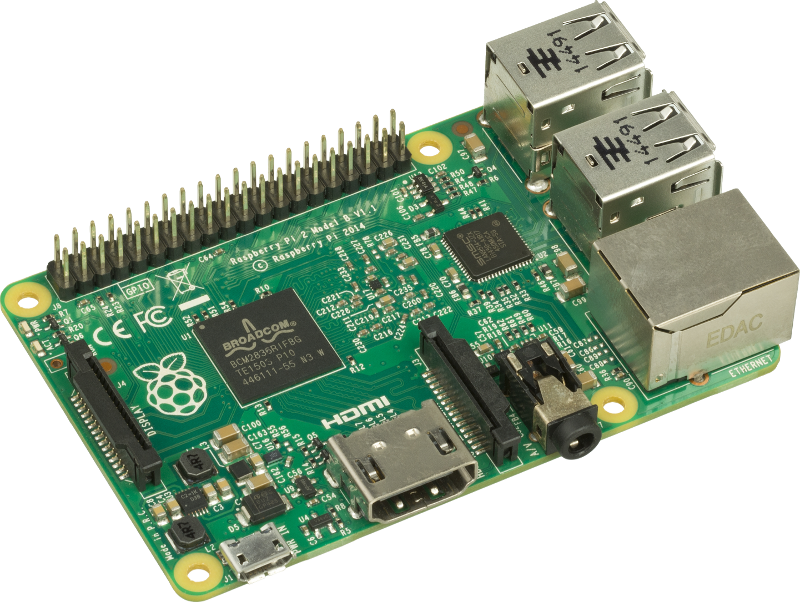
\includegraphics[width=0.56\textwidth]{res/raspberry}}
\caption{Raspberry Pi \cite{raspberry} with Broadcom System on Chip \label{fig:raspberry}}
\end{figure}
Actually almost all of the embedded systems use a SoC with similar boards, each one with its own size and configuration.

In order to accommodate many board implementations from different companies, each pin (or group of pins) of a SoC may have multiple configuration and operating modes.
The configuration of the pins is managed by the pin controller, a particular subsystem of a SoC.
Through a specific set of registers belonging to the pin controller, the system can configure the operating mode of the pins, such as their input or output mode.
These registers are typically accessible through a particular memory region called I/O memory. Such a kind of I/O access is known as \emph{Memory Mapped I/O}.

The features provided by a pin controller can be grouped into two main categories:
\begin{itemize}
	\item \itemname{pin configuration}: allows the system to change some electrical properties of the pins, such as direction, event detect, interrupt, etc.;
	\item \itemname{pin multiplexing}: each pin of the SoC may have many usages, also known as \emph{alternate functions}, depending on what is needed by the external board.
		The pin multiplexing feature enables the system to specify which type of function is needed on each pin.
\end{itemize}

As the I/O attack is a very low-level attack, it is necessary to dig further into the electrical world to know how these I/O interfaces work.


\subsection{SoC pins}
\label{sec:iopins}

I/O interfaces of a System on Chip provide a connection between internal modules and external electronic devices.
As shown in \myfig{fig:chips}, they are physically visible from the outside of the chip package,
usually in the form of pins \subref{fig:pins} or soldering balls \subref{fig:balls}.

\begin{figure}[h]
\centering

\begin{subfigure}{.45\textwidth}
\centering
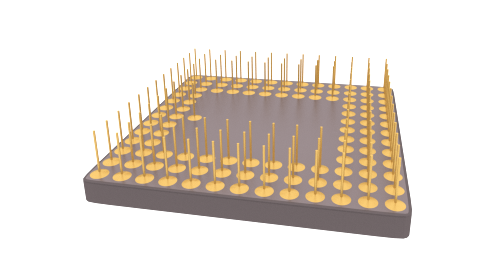
\includegraphics[width=\linewidth]{res/pins}
\caption{\label{fig:pins}}
\end{subfigure}
\begin{subfigure}{.45\textwidth}
\centering
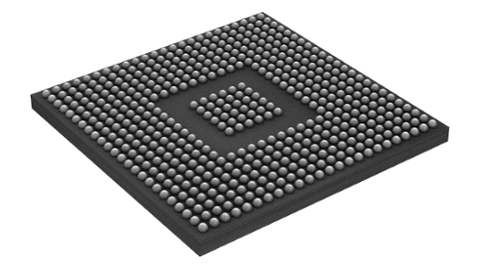
\includegraphics[width=\linewidth]{res/balls}
\caption{\label{fig:balls}}
\end{subfigure}

\caption{I/O connections packaged as \subref{fig:pins} Pin Grid Array and \subref{fig:balls} Ball Grid Array\label{fig:chips}}
\end{figure}

Internally they are connected to the silicon die through bonding wires, and are managed by a specific I/O circuit which may vary according to the specific chip.
Although there are many different implementations, almost all of the available SoCs have I/O ports with very similar functionalities.
For our purpose, we can describe them in an implementation-independent manner by using simplified generic schematics.


\subsubsection{Pin configuration}
\label{sec:pinconf}

The schematic depicted in \myfig{fig:pinconf} helps us to discuss about the first set of features: pin configuration.
The operation mode described in this section is also known as General Purpose I/O (GPIO).

\begin{figure}[h]
\centerline{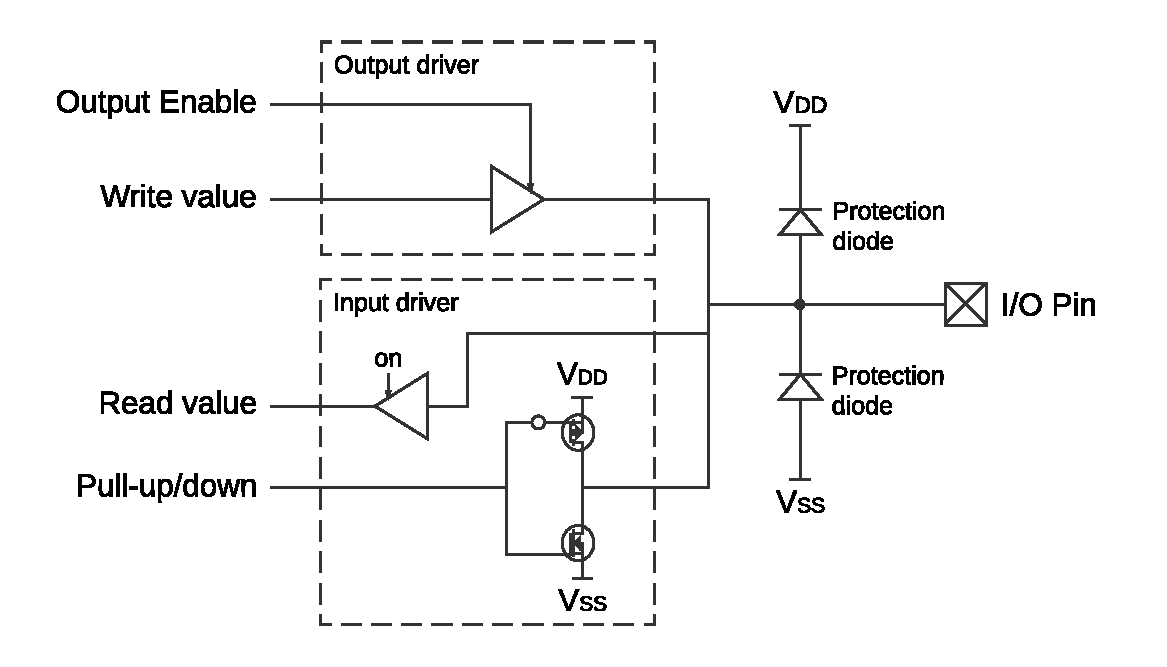
\includegraphics[width=0.8\textwidth]{res/pinconf}}
\caption{General Purpose I/O pin configuration circuit \label{fig:pinconf}}
\end{figure}

Apart from the protection diodes that serve as shield against input currents lower than $V_{SS}$ or higher than $V_{DD}$,
the circuit is divided into two different parts: one for output and one for input.
\begin{itemize}
	\item \itemname{Output driver}:
		The output module is basically a buffer controlled by an output enable signal.
		This signal controls the direction of the pin (input or output). If it is high, then the pin is in output mode
		and the value coming from a write operation goes through the buffer to the actual pin.
		If it is low, the pin is in input mode and the write signal is blocked, so it is not possible to change the external value of the pin from inside anymore.
	\item \itemname{Input driver}:
		The input driver has a similar buffer to read the value, usually having hysteresis capability which is useful for filtering unstable external values.
		Since the read buffer is always active, the input value is always available, even if the pin is currently working in output mode.
		The reason for this is merely physical: even if the external value was blocked by the buffer,
		one would always get a value by reading the input signal, because a value is nothing but an interpretation of the voltage level on a wire.
		When the pin is set as input, the pull-up/pull-down network enables the user to have a ``default'' value on the pin,
		namely a defined state maintained while the pin is not actively driven from outside. This feature is useful to avoid so called ``floating'' inputs.
\end{itemize}

For Pin Control Attack, what is more interesting about the circuit in \myfig{fig:pinconf} are the following two properties:
\begin{itemize}
	\item there is no checking about the input state, so it is possible to perform a read even when the pin is in output mode;
	\item vice versa, it is not possible to write to a pin which has been configured as output.
\end{itemize}

Furthermore, it is also possible to drive the pull-up/down network, factually disturbing the real value of the I/O pin in an unpredictable way.
Virtually, it is even possible to interfere with the pin value by means of external electromagnetic fields.
In these cases the effects strongly depends on the actual implementation of the printed circuit board as well as on the external components connected to the I/O pin.


\subsubsection{Pin multiplexing}

Inside a chip, each I/O pin may be connected to more than one device, which can be selected depending on the application
(\ie the way of soldering or wiring the package into an electronic board).
This SoC feature is known as pin multiplexing (also ball multiplexing, pad multiplexing, alternate functions).
Even though pin multiplexing is designed for hardware configuration, in almost all modern chips it is possible to change the function at run-time.

\begin{figure}[h]
\centerline{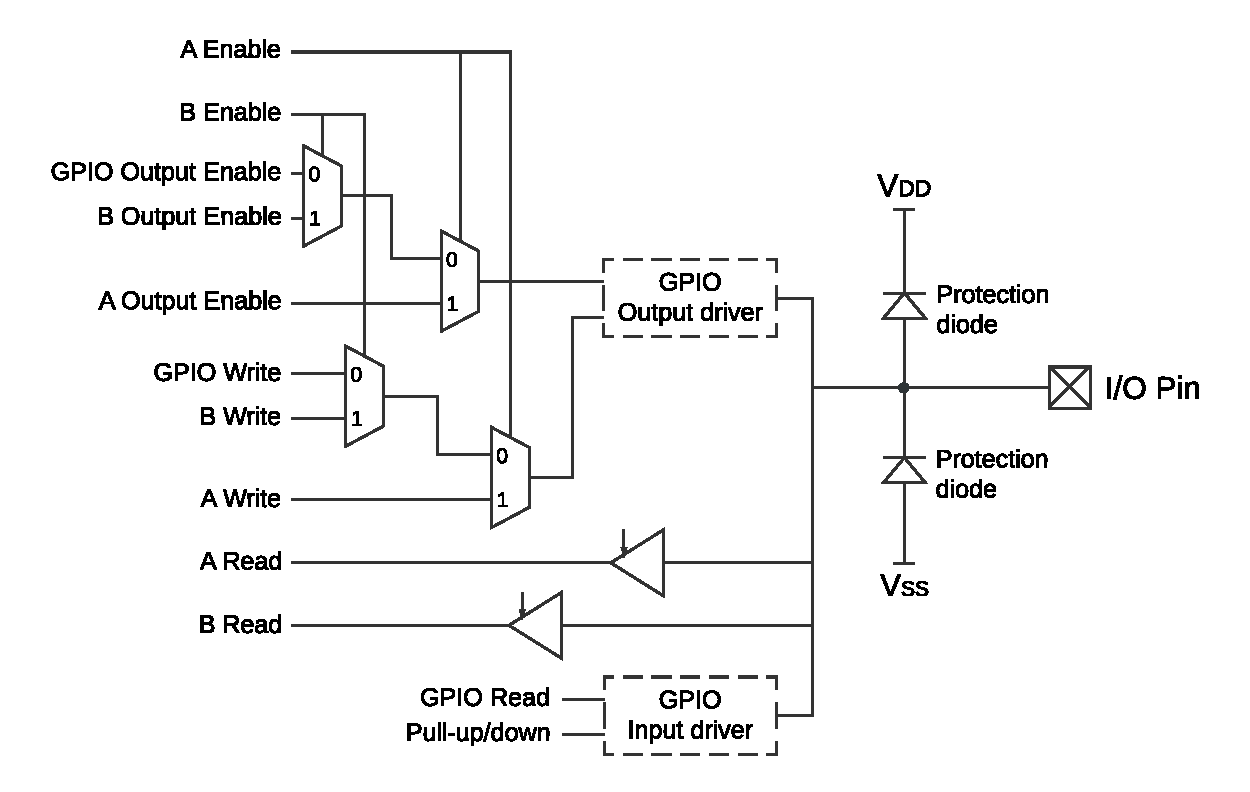
\includegraphics[width=0.8\textwidth]{res/pinmux}}
\caption{Generic I/O pin multiplexing circuit \label{fig:pinmux}}
\end{figure}

\myfig{fig:pinmux}~ shows a possible hardware implementation of pin multiplexing.
The I/O pin in the figure is connected to two different peripherals inside the chip, namely A and B,
and it is also accessible through basic GPIO as described in \mysec{sec:pinconf} above.
The access to the GPIO output driver is regulated by two in cascade multiplexers for each signal of the module.
If the peripheral A is enabled, then the signals driven by A go through the multiplexers and can drive the actual value of the pin,
while GPIO and peripheral B output signals are blocked. Instead, if only peripheral B is enabled then only its signals are able to reach the I/O pin.
Note that in this last case the peripheral A should not be enabled, because A multiplexers have precedence against B ones.
Thus, the cascading of multiplexers actually implements a priority mechanism between peripherals A and B.
If neither A nor B are enabled, then no alternate function is active for the I/O pin and it could be driven by GPIO signals.
Each peripheral may also have its own dedicated input line, to get values from the I/O port in the same way as GPIO does.

For our purpose, at least two interesting properties can be inferred from pin multiplexing schematic of \myfig{fig:pinmux}:
\begin{itemize}
	\item it is possible to block output signals from peripherals by simply changing the multiplexing configuration;
	\item the GPIO value can be read at any time, independently from the current multiplexing state of the output.
\end{itemize}


\subsection{PLC architecture}
\label{sec:plc_arch}

As introduced in \mychap{chap:intro}, Programmable Logic Controllers are a particular kind of embedded systems,
designed to work into harsh environments and to control a physical process, typically an industrial or other critical processes.
In this section we examine the hardware and the software architecture of a PLC. This analysis will be needed later to better explain
the threat model and the implementation of Pin Control Attack.


\subsubsection{Hardware architecture}

Since it is built for working into a rough environment, the internal hardware of a PLC is shielded and not directly visible as the Raspberry Pi one.
\myfig{fig:wagoplc} shows an example of a basic PLC, provided by Wago. This model will be later used for our tests.
Note that, although we provide this specific example, the basic concepts described here are still valid for most of the PLC on the market, unless otherwise specified.

\begin{figure}[h]
\centerline{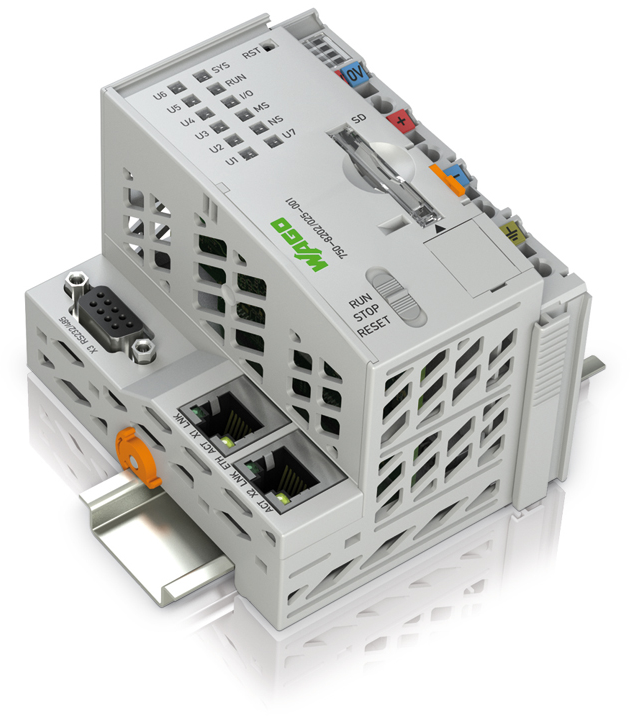
\includegraphics[width=0.5\textwidth]{res/wagoplc}}
\caption{PFC200 Programmable Logic Controller from Wago \label{fig:wagoplc}}
\end{figure}

Internally, the PLC has a System on Chip whose architecture is substantially equivalent to the one discussed in the above sections.
Therefore, the same concepts are applicable to PLCs as well.
Anyway, from our analysis we found that their architecture could be a bit more complicated with respect to a plain SoC.
Since the environment in which PLCs work may greatly differ case by case, they are designed to be as versatile as possible.
Vendors know that their PLC could be deployed in many different physical processes, possibly having completely diverse sensors and actuators to interact with.
Clearly, it is unreasonable to put every possible I/O interface on the same SoC. For this reason, most of the available PLCs comes with the possibility
of connecting a certain number of external components called \emph{I/O modules}. Each I/O module contains its own embedded SoC,
responsible for a specific subset of I/O interfaces (\eg digital input/output, analog input/output, pulse-width modulation, communication, etc.).
This hardware architecture is summarised in \myfig{fig:plc_arch}.

\begin{figure}[h]
\centerline{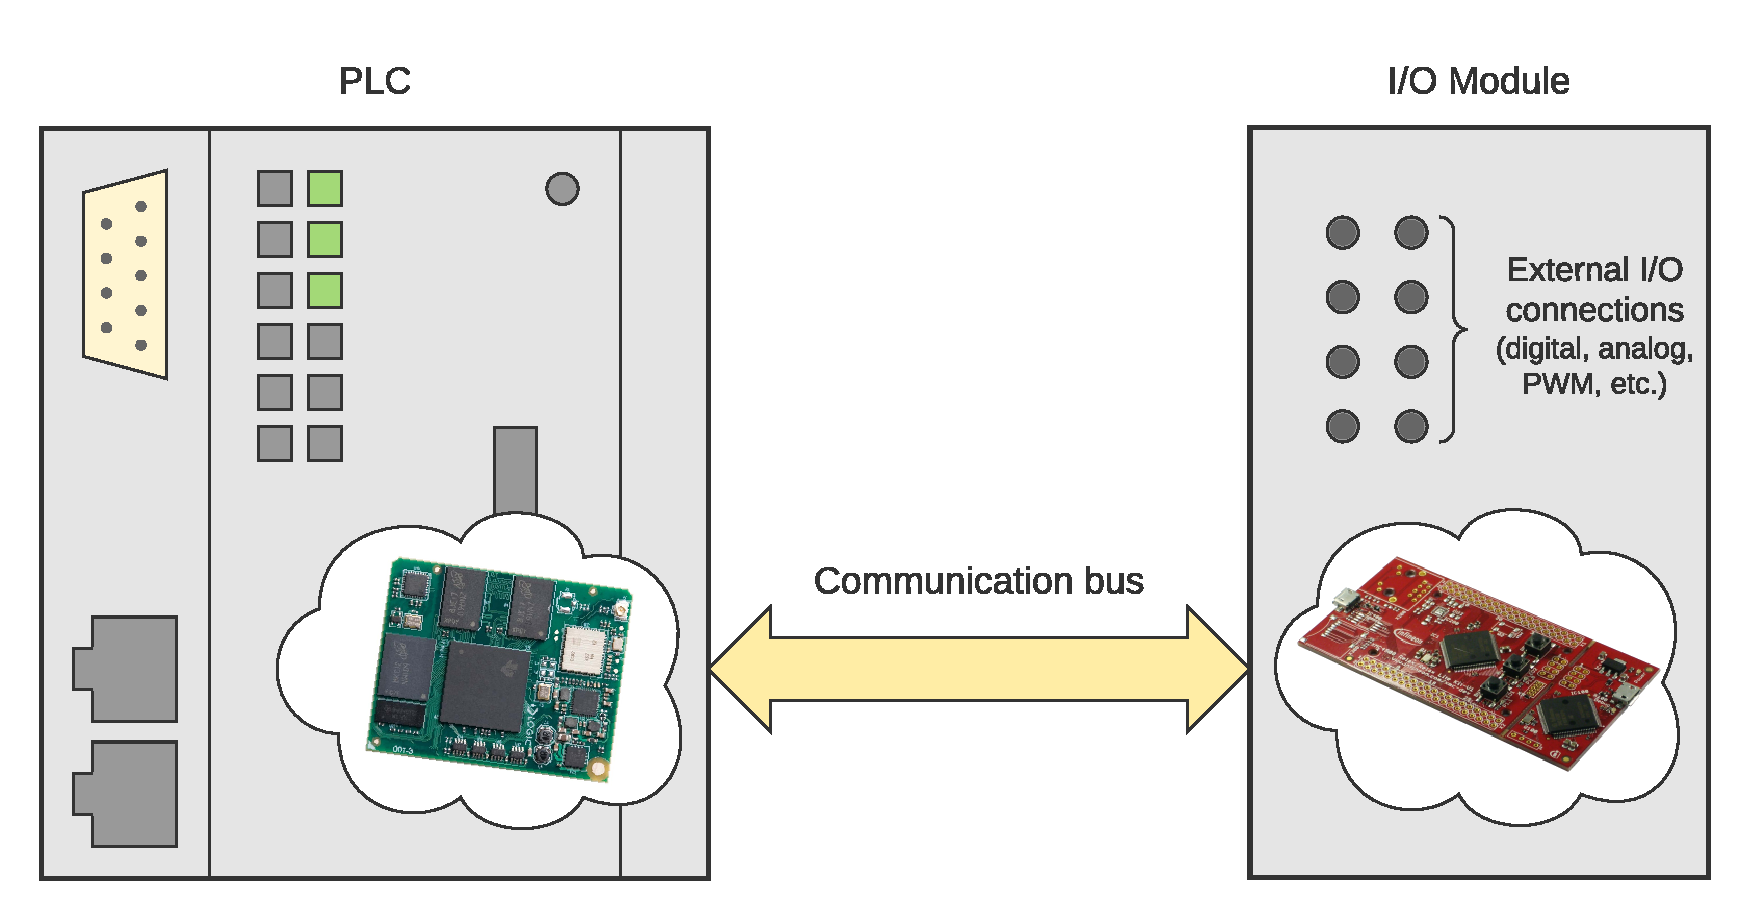
\includegraphics[width=0.8\textwidth]{res/plc_arch}}
\caption{PLC hardware architecture \label{fig:plc_arch}}
\end{figure}

The main portion of the PLC communicates with the I/O modules via a system bus, which is, in turn, connected to the I/O interfaces of the PLC.
This architecture with I/O modules adds one level of indirection between the targeted PLC and the external world, since there is another SoC in the middle.
Anyway, the same concepts of Pin Control Attack can be applied to such an architecture as well. It is sufficient to consider that the I/O interface of the PLC,
connected to the internal bus, is now the new direct target of our attack, while the final I/O becomes an indirect target. As we demonstrate in \mysec{sec:attack_plc},
by tampering with the I/O related to the communication bus it is possible to achieve equivalent results, proving that Pin Control Attack is still applicable on real PLCs.


\subsubsection{Software architecture}

The PLC typically comes with a real-time operating system (\eg Linux with RT-preempt patch, VxWorks etc.), because of the time requirements imposed by its main task.
Above the operating system, a software called \emph{PLC runtime} is responsible for managing the execution state of the control process and regulating the access to the PLC.
Through the runtime, the industrial operator can connect its terminal to the PLC and upload the desired control program, the \emph{logic}.
The PLC logic is the application code responsible for the control of the physical process, dealing with input and output interfaces.
As shown in \myfig{fig:plc_swarch}, this architecture can be divided into three layers, laying one above the other.

\begin{itemize}
	\item \itemname{Firmware}: the lowest layer, which basically corresponds to the operating system kernel. Although they are typically two distinct parts,
		here we consider the bootloader also as ``part'' of the firmware, because in this context their separation is irrelevant.
	\item \itemname{Runtime}: a software which is part of the application layer above the firmware, and it is started by the operating system itself.
	\item \itemname{Logic}: the control program running within the runtime environment. Its execution is started and stopped by the runtime,
		and its code is dynamic: it may change whenever the industrial operator decides to upload a new control program to the PLC.
\end{itemize}

\begin{figure}[h]
\centerline{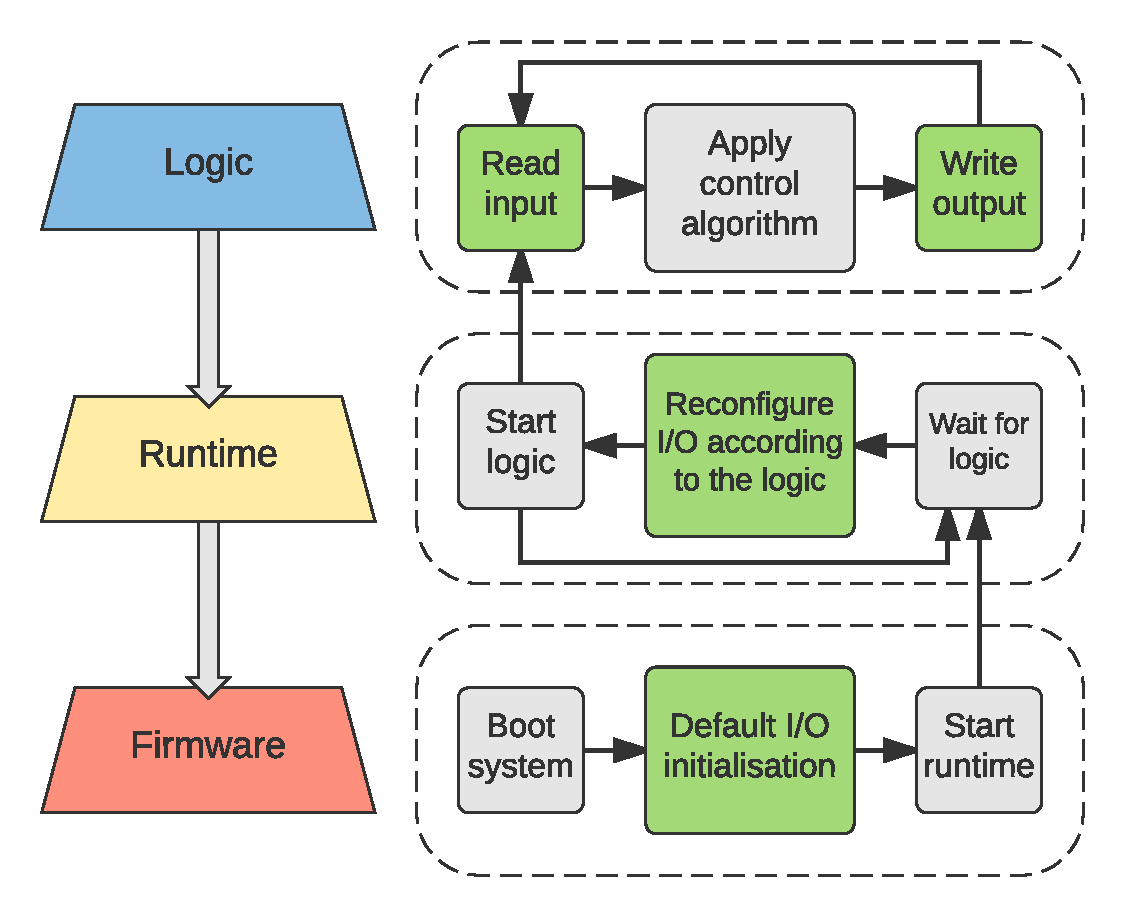
\includegraphics[width=0.7\textwidth]{res/plc_swarch}}
\caption{PLC software architecture \label{fig:plc_swarch}}
\end{figure}

\myfig{fig:plc_swarch} also summarises the execution flow of each layer, from bottom to top, highlighting (in green) the tasks directly related with the I/O.

When the firmware is loaded into memory and the system is booting, one of the early operation performed is known as I/O initialisation sequence.
In this phase, the drivers within the kernel configure their own I/O registers with their default values.
I/O initialisation includes both pin configuration and pin multiplexing. Normally, pin multiplexing is only performed at boot time, and, even though it is not forbidden,
pin multiplexing is never modified at run-time. Conversely, pin configuration may be changed later at run-time. Thus, depending on the implementation, the configuration
written during I/O initialisation may correspond or not to the one desired by the final application.

After the I/O has been initialised, the firmware loads the main application needed by the controller: the runtime.
The PLC runtime waits for a logic to be uploaded into the PLC from a terminal connected via the network interface.
The execution flow reported in \myfig{fig:plc_swarch} for the runtime layer is a general process, including the case when a PLC is started for the first time.
If a PLC is already in production, it is rarely restarted. However, when a reboot is needed (\eg for firmware update),
it may be configured to persistently save the current logic into a non-volatile memory and restore it after reboot.
In this case the ``Wait for logic'' step in \myfig{fig:plc_swarch} can be simply skipped, because a logic may be already available from disk.

When a logic is available, from network or from disk, the PLC runtime analyses its content.
The I/O configuration expected by a specific logic is bundled with the logic itself, because it is decided by the operator who has knowledge of the physical process
and knows how sensors and actuators are connected to the PLC I/O ports. With respect to the hardware architecture shown in \myfig{fig:plc_arch},
a change in the input/output required by the operator is actually reflected into a configuration change of the external I/O modules.
Whether this process involves a change in the I/O configuration of the PLC itself depends on the implementation and on the modification extend
(\eg if a new I/O module has been attached, this will probably require a change in the communication protocol and so on the I/O interface of the PLC).
After the new I/O configuration has been applied, the logic can be executed. From an operating system point of view, the logic is running in the same context of the PLC runtime.

As briefly discussed in \mychap{chap:intro}, the PLC logic executes the main \emph{scan cycle}. For each iteration, it reads from inputs, executes the control algorithm,
and writes to outputs. The control algorithm has been programmed by the industrial operator, and loaded through the interface provided by the PLC runtime.
When the logic is running, input and output pins have already been configured by the runtime, and the logic assumes that the I/O configuration does not change during its execution.
Both the logic and the runtime interacts with the I/O, but in different ways. The runtime deals with I/O configuration registers, while the logic performs read/write operations
related to I/O values. Both kind of interactions, anyway, require the same privileges, which will be later leveraged by Pin Control Attack.


\section{Attack Design}

Given the properties discussed in \mysec{sec:embed_arch}, it is possible to misuse the registers used to configure I/O peripherals,
and that is what Pin Control Attack does. This can happen at run-time, during the execution of the controller on a real process,
without any reaction from the PLC runtime or the operating system, thus remaining completely stealth.

We can argue that Pin Control Attack is actually applicable on any System on Chip having the
architecture described in \mysec{sec:embed_arch}. However, PLCs represent a particularly interesting target among all the embedded systems based on SoC.
PLCs leverage the interfaces of a SoC to interact with sensors and actuators, having direct effects on our physical world.
Therefore, if the I/O of a PLC is compromised, this constitutes a much more significant security and safety risk with respect to other
non-critical embedded system. For this reason, PLCs represent one of the most attractive targets for Pin Control Attack.

In this section we focus on the design of I/O attack. First, we summarise the host-based detection mechanisms taken into account
during the attack design and the techniques used to evade them. Second, we analyse the attack itself in more detail.
The goal of this chapter is to help us having a better understanding of the attack, and to provide a detailed threat model on which our defense design will be based on.

Pin Control Attack has been designed to be different from previous attack techniques, and to circumvent the off-the-shelf host-based detection systems.
The authors of I/O attack have identified two main defensive mechanisms whose properties makes them more easily applicable to PLCs.
Here we want to generalise and consider them in our threat model, clarifying how and when Pin Control Attack becomes applicable and interesting for attackers.
We also show how these defenses are circumvented by Pin Control Attack, and describe the available attack techniques.
We do not repeat here the detailed description made in \cite{ghostplc}. We only want to have basic concepts definition,
in order to be able to focus on our further analysis and implementation of the attack.


\subsection{Defense analysis}
\label{sec:def_analysis}

At this point, one could ask why descending to the lowest level possible to conduct an attack, when a lot of easier techniques (\eg function hooking) may achieve equivalent results.
The point here is that many producers of embedded systems and PLCs already started to move towards a more security-aware production.
As considered in \cite{ghostplc}, in order to be applicable to PLCs, a defensive mechanism should have at least the following properties:
\begin{itemize}
	\item low CPU overhead: CPU resources are limited in embedded systems such as PLCs, which typically have hard real-time constraints;
	\item designed to run on an operating system: almost all of the modern PLCs have a real-time OS running on it;
	\item no hardware modification required: many solutions are hardware-based \cite{trustlite,hardware-ibmac,ocfmm,fine-grained,bb-cfi}, making them not easily applicable;
	\item no virtualisation required: the majority of embedded systems, like PLCs, does not support virtualisation;
		thus solutions like \cite{hypervisor-control} are less attractive.
\end{itemize}

Given these considerations, we can list some of the applicable defenses:
\begin{itemize}
	\item \itemname{SEM}: the Symbiote detection system described in \cite{symbiotes}, which protects the kernel from code modification attacks;
	\item \itemname{Autoscopy Jr.}: the lightweight intrusion detection system proposed in \cite{autoscopy}, effective against control flow manipulation inside the kernel.
\end{itemize}

The above detection systems still have some shortcomings, leveraged by Pin Control Attack.
First, they are based on a comparison with golden references (the symbiotes and the TLL, respectively) taken from a subset of the entire kernel space.
If the attacker is able to find a portion of the kernel space which has not been considered by the detection system, then it can be circumvented.
For example, Autoscopy Jr. can be bypassed if the attacker is able to craft a duplicate of the kernel functions it needs.
If a duplicate function is used instead of the original version, Autoscopy Jr. does not throw an alert, because this function is not listed in the TLL at all.
Second, the references used by both defenses are \emph{static}, which means that they are based on previous analysis of the immutable (static) portion of the system.
Thus, an attacker could still use dynamic memory, whose content changes during run-time, to conduct its own attack.
In the case of SEM, only static code regions (which are immutable) are taken into account, so any malware placed in dynamic memory will not be detected.
Autoscopy Jr., instead, considers the function pointers used inside the kernel, including the ones inside the System Call Table and other similar tables.
Therefore, it is able to detect only \emph{data hooks} but not \emph{code hooks}; in other words, any direct code modification (\eg of the kernel text) is still possible.

Anyway, these two defenses may be used in combination, thus providing a host-based IDS able to detect both code and data hooks.
Even if they are deployed together, however, attacks through dynamic memory and without function hooking are still possible,
since monitoring dynamic memory is a far more complex issue. One of the implementations of Pin Control Attack (see \mysec{sec:attack_impl})
leverages exactly the kernel dynamic memory to reach its purpose.

Host-based detection mechanisms like the ones discussed above will likely be deployed into many commercial products within the next years \cite{symbiote_web, autoscopy_web},
raising the bar for attackers. Therefore, Pin Control Attack will become more and more interesting as long as classical techniques (\eg function hooking) are overcome.


\subsection{Threat model}
\label{sec:threat_model}

In our work, we assume that the system is protected at least by the HIDSs described in \mysec{sec:def_analysis}, or equivalent.
Hence, we assume that the attacker cannot tamper with operating system (kernel) functions and data structures, but it can still use dynamic memory to insert its malicious code
and tamper with the I/O configuration. The attacker can also write its own version of kernel functions if needed, and call them separately in order to avoid HIDSs.
This approach, anyway, requires very high effort and would really be the last option for an attacker.

The attacker, depending on the attack implementation, may need different running privileges on the target system to execute Pin Control Attack.
Generally speaking, the minimum privilege required is the privilege level of the PLC runtime, which has access to the I/O configuration registers.
As already discussed in \cite{ghostplc}, many ICS-CERT advisories have shown that PLCs have vulnerabilities that could lead to malicious code execution
\cite{plc-network,abb-codesys,codesys-server,schneider-bof,rockwell-vuln,rockwell-vuln2}, and they may affect PLC runtime software as well.
Thus, obtaining the same PLC runtime privilege level is feasible on real systems.

As in \cite{ghostplc}, we assume that the attacker knows both the physical process controlled by the target system and the mapping
between I/O configuration and external sensors and actuators. The former is typically known by the attacker, which has reasonably studied its target before conducting the attack.
This is confirmed by Stuxnet \cite{stuxnet}, where attackers had very deep knowledge of target system and physical process.
The latter is given by a knowledge of the PLC logic, which, as said, already comes with the mapping between I/O interfaces and control variables used by the logic.
Furthermore, the research presented in \cite{dynamic-payload,sabot} shows that it is possible to infer the structure of the devices connected to the PLC and used by the logic,
factually lowering the bar for attackers which do not need an a priori knowledge of the I/O mapping anymore.


\subsection{Pin Control Attack}

Based on the previous assumptions, Abbasi et al. \cite{ghostplc} crafted Pin Control Attack, which is capable of manipulating the physical process
controlled by a PLC without requiring any firmware or logic modification.
The idea of Pin Control Attack is that the attacker operates at the lowest level possible, targeting the interaction
between the firmware and the I/O, as shown in \myfig{fig:target}. For this reason, the attack is also known as I/O attack.
Despite its crucial function in embedded systems, I/O hardware architecture and I/O drivers are currently designed
without taking into account any concept of security, assuming that I/O is reliable. Unfortunately, given the properties inferred in \mysec{sec:embed_arch}
from a generic hardware architecture, this is often not the case.

\begin{figure}[h]
\centerline{\includegraphics[page=6,viewport=50 620 300 750,clip]{res/ghostplc}}
\caption{Pin Control Attack target, from \cite{ghostplc} \label{fig:target}}
\end{figure}

As described in \cite{ghostplc}, Pin Control Attack is designed to evade off-the-shelf HIDSs presented in \mysec{sec:def_analysis}.
In particular, it leverages kernel dynamic memory (in one implementation variant) or it uses a simple user code (in a second variant).
Both variants are able to circumvent the above detection mechanisms.

The authors of \cite{ghostplc} have found at least two different attack vectors for Pin Control Attack: \emph{Pin Configuration} and \emph{Pin Multiplexing}.
Both kind of attacks leverage the SoC properties described in \mysec{sec:embed_arch}.
The attack is performed by misusing the control registers used to program the I/O peripherals, writing malicious values into them.
If the attack targets I/O configuration registers, it is a Pin Configuration Attack, otherwise, if the targeted registers are related to the multiplexing state of the pins,
then it is a Pin Multiplexing attack. In some architectures, I/O configuration and multiplexing is achieved by using the same set of registers
(\eg different bits of the same register may have different purposes).

In both cases, the main principle behind the attack is something that they called \emph{memory illusion}, which is represented in \myfig{fig:illusion}.
In a system equipped with a Memory Management Unit (MMU), that is the most common scenario for PLCs, each process cannot directly access to physical address space.
Every memory access is mediated by the MMU, which creates an abstraction called \emph{virtual address space}, or \emph{virtual memory}.
When a process wants to access physical memory, it has to request a mapping to the system between physical address space and virtual address space.
In this way, every process has its own ``virtual view'' of the physical memory. This is valid also for I/O memory, which is part of the physical memory.
Once a mapping has been established, the I/O can be managed by accessing the mapped virtual memory.
\begin{figure}[h]
\centerline{
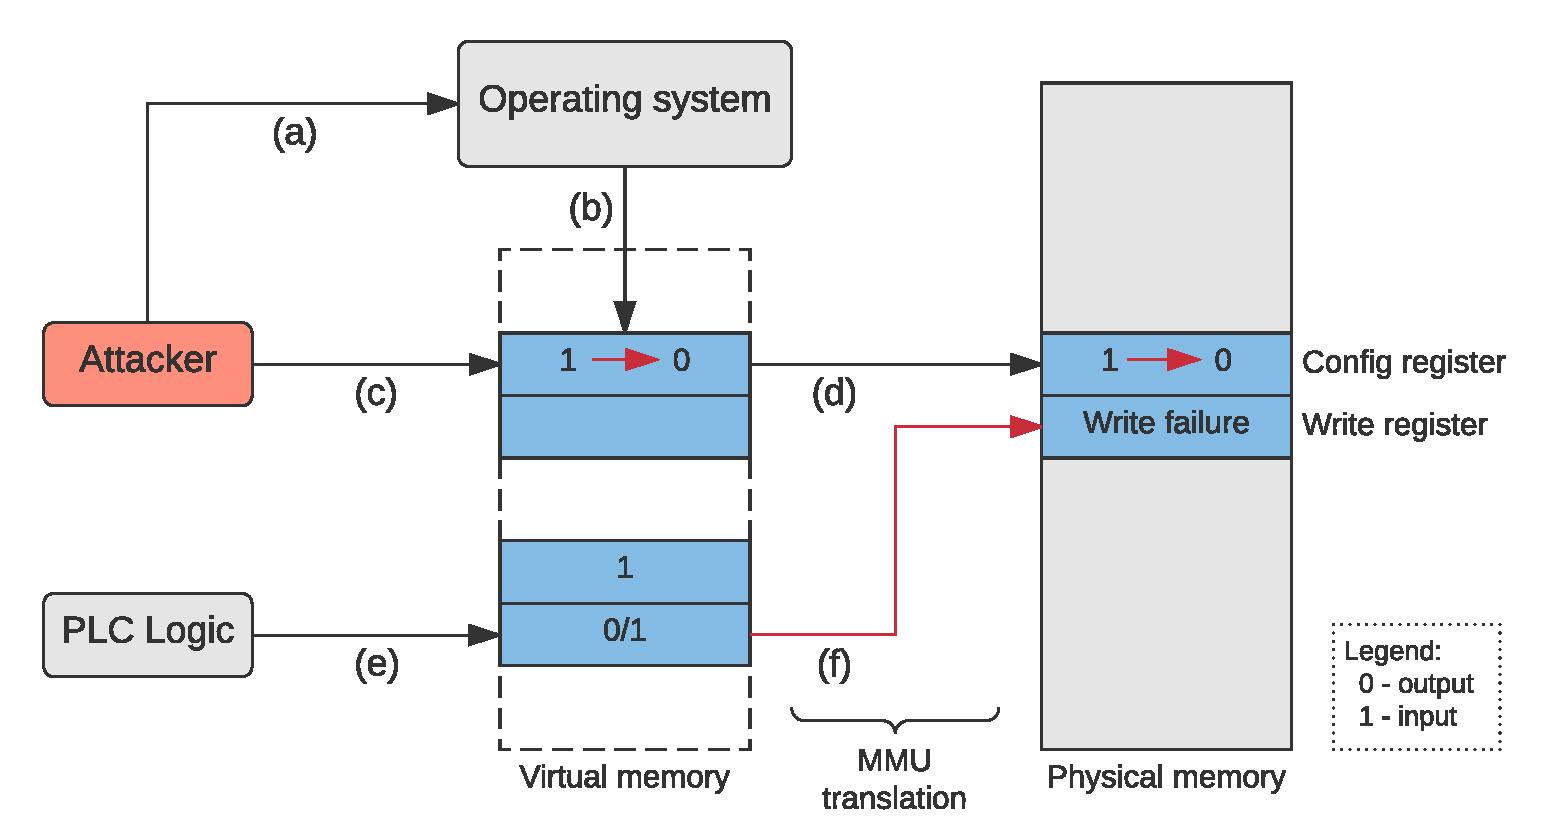
\includegraphics[width=0.9\textwidth]{res/illusion}}
\caption{Pin Control Attack memory illusion \label{fig:illusion}}
{\phantomsubcaption\ignorespaces\label{fig:mapping_request}}
{\phantomsubcaption\ignorespaces\label{fig:mapping_provided}}
{\phantomsubcaption\ignorespaces\label{fig:conf_change}}
{\phantomsubcaption\ignorespaces\label{fig:phys_change}}
{\phantomsubcaption\ignorespaces\label{fig:virt_write}}
{\phantomsubcaption\ignorespaces\label{fig:write_failure}}
\end{figure}
Thus, as \myfig{fig:illusion} outlines, an attacker can do the following: first, it has to request a mapping for I/O memory \subref{fig:mapping_request};
once a virtual mapping is provided by the operating system \subref{fig:mapping_provided}, the malicious process is able to alter the pin configuration (\eg change an output pin to input)
through virtual memory \subref{fig:conf_change}. This change is immediately reflected into physical memory via MMU translation \subref{fig:phys_change}. When the PLC logic,
which is a normal process in the system, tries to update the value of the pin through virtual memory \subref{fig:virt_write},
the target address of the write instruction arrives to the MMU, which translates it to the corresponding physical address.
Unfortunately, since the pin has been changed to input, the execution of the instruction does not actually affect physical memory \subref{fig:write_failure}.
Therefore, the write silently fails, but no signal error is reported back to the CPU, and from the process virtual perspective everything went correctly.
As explained later in \mychap{chap:defense}, the fact that the virtual address of the instruction actually reaches the MMU will be a crucial mechanism
for the design of our defense.

As reported in \cite{ghostplc}, only by leveraging the configuration of pins they crafted an attack which is able to do the following:
\begin{itemize}
	\item reconfigure an I/O pin as input when the PLC logic is attempting to write;
	\item reconfigure an I/O pin as output and write a malicious value when the PLC logic is attempting to read.
\end{itemize}
In this way, the attacker can disable specific output operations and feed the PLC logic with malicious input at the same time.
In other words, Pin Control Attack takes the whole PLC logic as a black box. Instead of altering the logic code, it simply controls input and output values
by means of the above operations. Whether this approach can lead to useful results (for the attacker) is highly dependent on the actual PLC logic and, of course,
on the attacker purpose. In \mysec{sec:attack_pi} we show that this mechanism may be very interesting for the attacker, and we also discuss
about some hardware limitations of this approach.

Moreover, we imagine that many other attack possibilities may exist. An attacker can tamper with the I/O configuration in many other ways depending on the
specific I/O peripheral and on its features (\eg event detect, interrupts, clock signals, etc.), and the effects of the attack are unpredictable.
If the attacker can analyse the reference manual of the target SoC (mostly publicly available) and it has enough competence and time,
the only limit to Pin Control Attack becomes fantasy.
To give an idea of what such an attack can do, imagine a simple SoC pin which can be multiplexed between a memory controller and a PWM controller.
If this pin is actually connected to an external memory, thus multiplexed to a memory controller, a Pin Multiplexing attack can lead to dangerous signals
sent from a PWM controller to a memory module, which may burn the memory. Furthermore, if a subset of pins is multiplexed to a specific controller (\eg I2C, SPI, DMA, etc.),
the control registers of the device can be targeted as well, obtaining an indirect effect on the corresponding I/O pins.

On the other side, from our analysis on a real PLC, we found that another attack vector is viable at a different abstraction level than hardware configuration.
Commonly, the I/O peripherals are controlled by operating system drivers, which in turn are used from user space applications like the PLC runtime.
As we show in \mysec{sec:attack_plc}, an attacker can target these drivers, or even these applications, to obtain equivalent effects without dealing with
the underlying hardware and I/O registers directly.


\section{Attack Implementation}
\label{sec:attack_impl}

In this section we first describe the available implementation presented in \cite{ghostplc}, which was the starting point of our analysis.
Next, we introduce a possible attack implementation on a real PLC. Both implementations are designed for Linux-based systems, and they have two different
variants: kernel side and user side. Each variant imposes different requirements for the attacker, which will be discussed in more detail in the next sections.


\subsection{Raspberry Pi}
\label{sec:attack_pi}

The system used for our experiments with the first implementation is a \emph{Raspberry Pi 1 Model B} based on an ARMv6 architecture, running the following kernel:
\begin{Verbatim}[fontsize=\small]
	Linux raspberrypi 4.4.22+ #912 Mon Sep 26 19:00:13 BST 2016 armv6l GNU/Linux
\end{Verbatim}
The Raspberry Pi 1 features a Broadcom System on Chip named \emph{BCM2835}. With reference to the BCM2835 documentation \cite{bcm2835},
we set up the system I/O by connecting a button as input, an LED and a servo motor as outputs. Button and LED are accessed via $2$ GPIO interfaces,
one configured as input and one as output, respectively. To connect the micro servo, we needed an external PWM controller. The controller is attached to the system
through the I2C interface, which requires two pins: one for the data line, \emph{Signal DAta} line (SDA), and one for the clock line, \emph{Signal CLock} line (SCL).
The resulting system on which we conducted our experiments is shown in \myfig{fig:pi_system}, and its I/O configuration is summarised in \mytab{tab:pi_pins}.

\begin{figure}[h]
\centerline{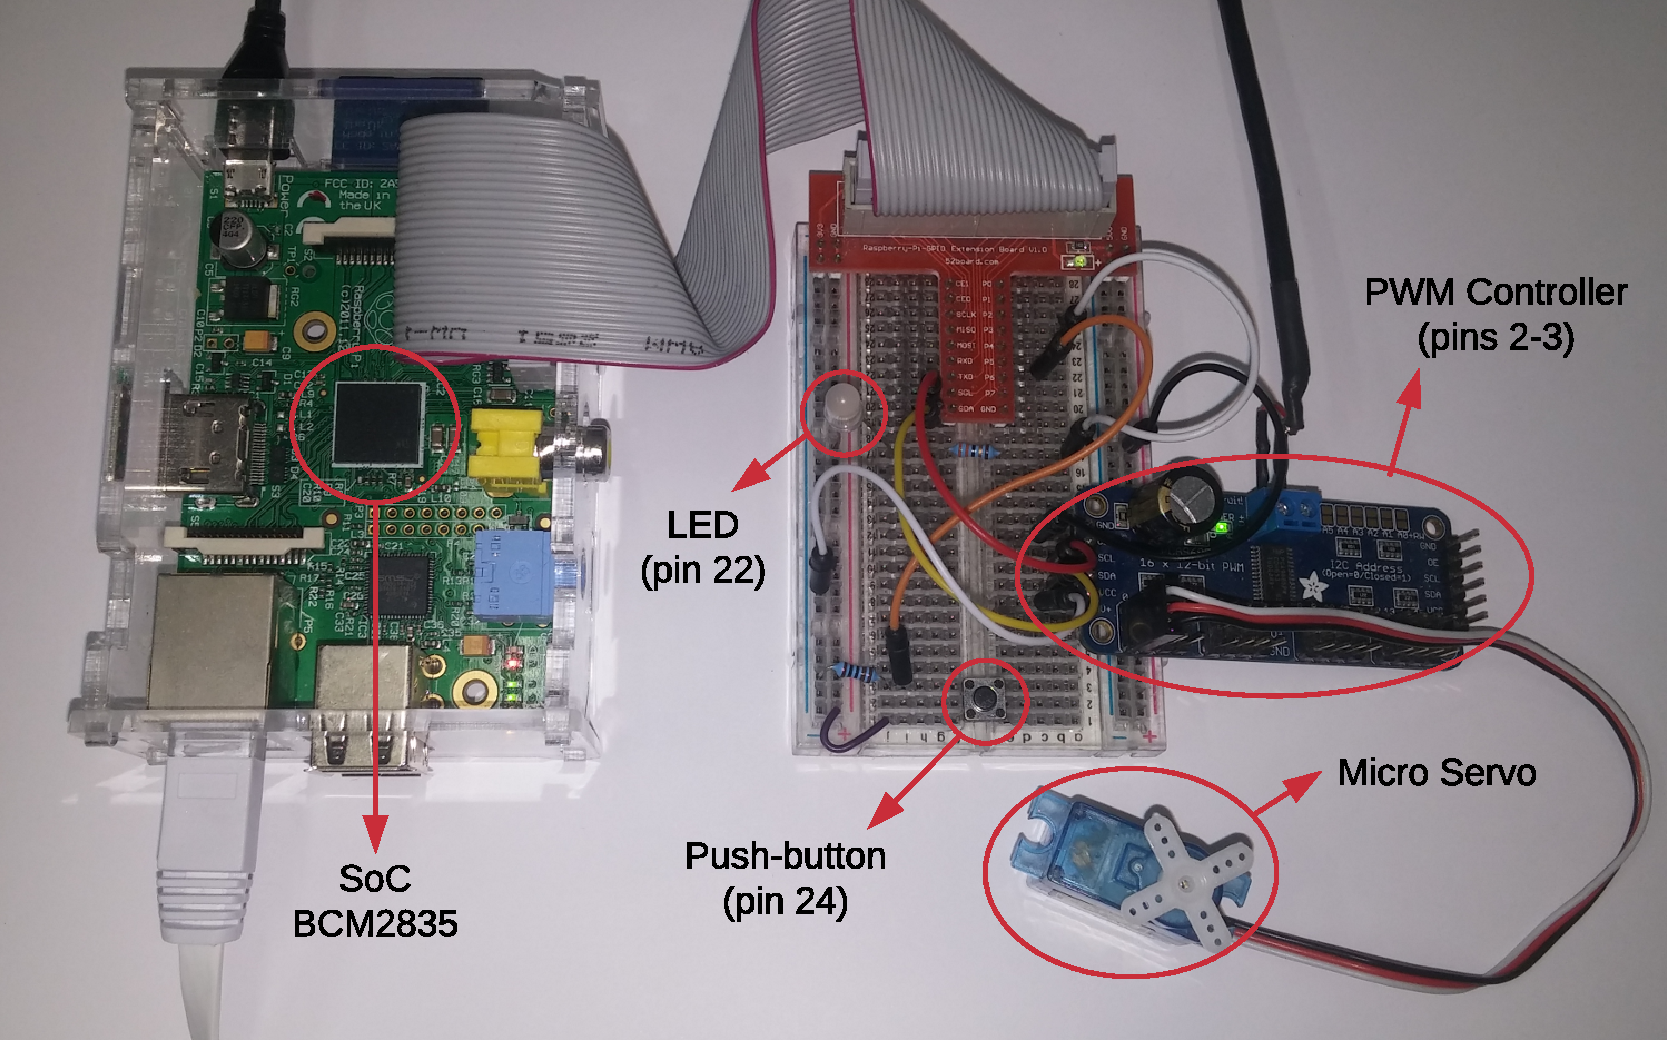
\includegraphics[width=0.8\textwidth]{res/pi_system}}
\caption{Raspberry Pi system used for experiments \label{fig:pi_system}}
\end{figure}

\begin{table}[h]
\centering
\renewcommand{\arraystretch}{1.5}
\begin{tabular}{|c|c|c|c|}
\hline
\thead{Pin} & \thead{Multiplexing} & \thead{Configuration} & \thead{Connected to} \\
\hline
24 & GPIO & Input & Button \\
\hline
22 & GPIO & Output & LED \\
\hline
2 & I2C SDA & - & PWM controller (servo) \\
\hline
3 & I2C SCL & - & PWM controller (servo) \\
\hline
\end{tabular}
\caption{I/O configuration of our Raspberry Pi testing system}
\label{tab:pi_pins}
\end{table}

To enable PLC capabilities on such a system, we installed a PLC runtime on it. In particular, we used \emph{CODESYS Control for Raspberry Pi SL}
provided by 3S-Smart Software Solutions GmbH \cite{codesys_runtime}. Through the CODESYS Development System \cite{codesys_dev},
we designed the PLC logic shown in \myfig{fig:pi_logic}, whose code is executed for each scan cycle.
\begin{figure}[h]
\centerline{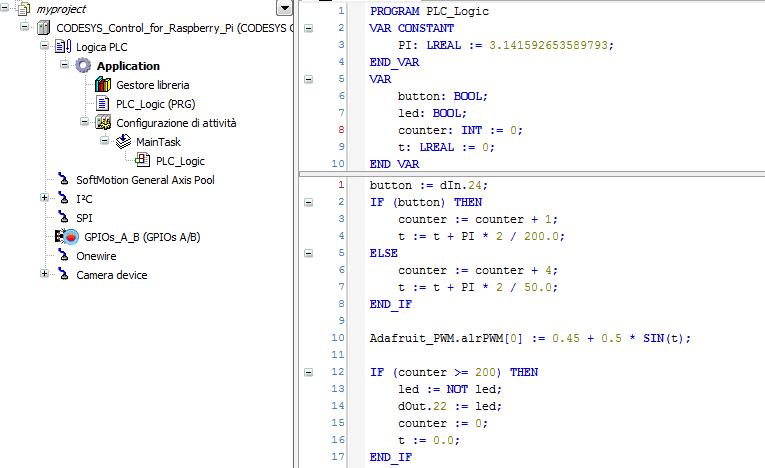
\includegraphics[width=0.8\textwidth]{res/pi_logic}}
\caption{PLC logic loaded into Raspberry Pi \label{fig:pi_logic}}
\end{figure}
We chose a $\SI{10}{ms}$ scan cycle interval, however, since this PLC runtime is not real-time, the timing may be affected by small errors ($\approx \SI{50}{\micro s}$). 
At each scan cycle, the logic reads from pin 24 (push-button), and writes the outputs accordingly.
The motor is driven with a sinus wave which makes it going forward and backward in the interval $[\SI{-45}{\degree}, \SI{+45}{\degree}]$.
If the button is not pressed, which corresponds to value $1$ (high), the LED is toggled every $2s$ and the motor completes a round in $\SI{2}{s}$.
If the button is pressed, that is value $0$ (low), both LED and motor frequencies are multiplied by $4$, and the new round time becomes $\SI{500}{ms}$.
The timing of the write operations, which is a multiple of the scan cycles, is controlled by software counters embedded into the logic.
Thus, while the input is high the counters are updated at normal speed; while the input is low they get updated $4$ times faster.
Furthermore, the logic does not write to the outputs at each scan cycle, but only when their values change (\eg the LED pin is written only every $\SI{2}{s}$).
This is typically different from the normal behaviour of a real-time PLC, as discussed in \mysec{sec:attack_plc}.

Given the system above, a possible implementation of Pin Control Attack can target input or output pins, having different effects.
By re-configuring an output pin as input, it is possible to disable the PLC logic write operations, leading to a Denial of Service (DoS) condition.
More interesting, by changing an input pin into output and writing its own values, an attacker can actually control the behaviour of the outputs.
In our case, if the attacker is able to intercept PLC logic read operations and write its own values, he can actually decide the frequency of the outputs.
For instance, as demonstrated by our attack experiments, if the attacker feeds the logic with $0$ and $1$ alternatively at each scan cycle,
the round time of the outputs becomes the average between $\SI{2}{s}$ and $\SI{500}{ms}$, factually having a frequency that is not even programmed into the logic.
But there is a limitation to this attack approach, implied by the architecture described in \mysec{sec:pinconf} and confirmed by the experiments:
the read operation is not reliable if the pin is configured as output pin. In our case, if we reconfigure pin 24 as output, the malicious value written into the write register
is not always the same value read by the PLC logic. That is probably because the voltage on the pin is actually driven by two entities at the same time,
the external sensor (the button) and attack code, so it is not deterministic whether, at the time of reading the pin level register, the voltage is considered a $1$ or a $0$.

The authors of Pin Control Attack described two different ways of intercepting read (or write) operations, and they implemented them into the following attack variants:
\begin{enumerate}
	\item a Linux loadable kernel module which is able to intercept logic read and write operations by leveraging the \emph{Debug subsystem};
	\item a user code which maps the physical I/O memory, or re-use PLC logic mapping, and manually watches the I/O values to synchronise itself with the PLC logic operations.
\end{enumerate}
Once the target operation has been caught, the attack modifies the I/O configuration according to its purpose.
Both implementations are able to evade the HIDSs analysed in \mysec{sec:def_analysis}, because they reside into kernel and user dynamic memory, respectively,
and they do not alter any control flow. Here follows a brief description of these two possible implementations, focused on the findings of our experiments.
For a more detailed analysis of the original version of the attacks refer to \cite{ghostplc}.


\subsubsection{Kernel module}
This variant requires root privileges, in order to be able to insert a loadable module into the kernel.
The kernel module makes use of debug registers, available in many embedded architectures, to catch PLC logic operations.
A debug register takes a virtual address, and optionally a process context, and raises a CPU exception when the address is accessed within the given context.
The access type may be read, write or execute: the first two are intended for data addresses, the last one for instruction addresses.
Thus, to use a debug register, the attacker needs to know the mapped virtual address used by the PLC logic to read/write the I/O pins.
These addresses are typically mapped by the PLC runtime before starting the logic, and can be easily obtained by looking into the \verb|/proc/<pid>/maps|
file, which lists the current mappings owned by a process identified by \verb|pid| (process id).
As discussed in \mysec{sec:threat_model} the attacker needs to know the running PLC logic, and the mapping between the I/O pins and
the physical process he wants to tamper. With reference to our target system, if the attacker knows that the input button is connected to pin $24$
and wants to intercept a read operation, then he can get the physical address of the read register from the SoC documentation \cite{bcm2835} (\verb|0x20200034|),
and finally the virtual address from the current PLC runtime mappings (\eg \verb|0xb6f40034|). With this information, he can install a debug exception handler
by setting a debug register: the malicious handler will be called whenever the PLC logic tries to read from that address.
Inside the handler, the attacker can decide whether to change the pin configuration and which value wants to feed the PLC logic with.
The use of debug registers gives the attacker a great timing accuracy on read and write operations,
but the overhead may be detectable by power consumption-based intrusion detection systems.


\subsubsection{User code}

This version does not need root privileges as the previous one. Since it is executed from user space, to have access to the I/O physical memory it needs to either
request a new mapping to the kernel or use the existing mapping of the PLC runtime. In both cases, the requirement is to have the same privilege level of the PLC runtime,
and this may be obtained by exploiting a code execution vulnerability affecting the CODESYS PLC runtime \cite{abb-codesys,codesys-server}.
The requirement needed to obtain the PLC runtime mapping is the same as the kernel module variant.
To intercept read and write operations, the attacker cannot use debug registers, because the access to the debug subsystem is mediated by the kernel \verb|ptrace| API.
Therefore, this version can only monitor the value of an output pin to get the relative time, and also infer timing information of other pins
by using its knowledge of the PLC logic. In our case, if the attacker monitors the pin $22$, when its value changes he knows from the logic
that at the same time the button input has been read, and the servo motor has just finished a round.
This information can be used to set relative timers, which will be activated on the next I/O events.
If the target system has real-time capabilities, as almost all real PLCs do, this technique can be even more accurate than our experiments in a non real-time environment.
Moreover, its overhead is much less than the corresponding debug register one, and it may not be easily detectable.


\subsection{PLC}
\label{sec:attack_plc}

As done for Raspberry Pi, we analysed a real PLC and considered the attack possibilities on this system as well.
The provided PLC is a \emph{PFC200 750-8202} model from \emph{Wago} vendor. It runs a Linux kernel with the RT-preempt patch, which gives it hard real-time capabilities.
In particular, the system runs the following kernel version on an ARMv7 architecture:
\begin{Verbatim}[fontsize=\small]
  Linux PFC200-4106BA 3.18.13-pfcxxx-02.00.02_00+14-rt10 #1 PREEMPT RT armv7l GNU/Linux
\end{Verbatim}
Furthermore, Wago gives complete (root/kernel) access to its system, and the user can even program its own PLC runtime \cite{wago_linux}.
As discussed in \mysec{sec:plc_arch}, different kind of I/O modules can be attached to the PLC. For our analysis, we attached a Digital I/O module to the communication bus.
PLC and I/O module are based on an \emph{AM3517} SoC from \emph{Texas Instruments} and an \emph{XE164} SoC from \emph{Infineon}, respectively.
The digital I/O module has $16$ different pins, $8$ for input and $8$ for output, and we connected a button as input and an LED as output,
obtaining the system shown in \myfig{fig:plc_system}.

\begin{figure}[h]
\centerline{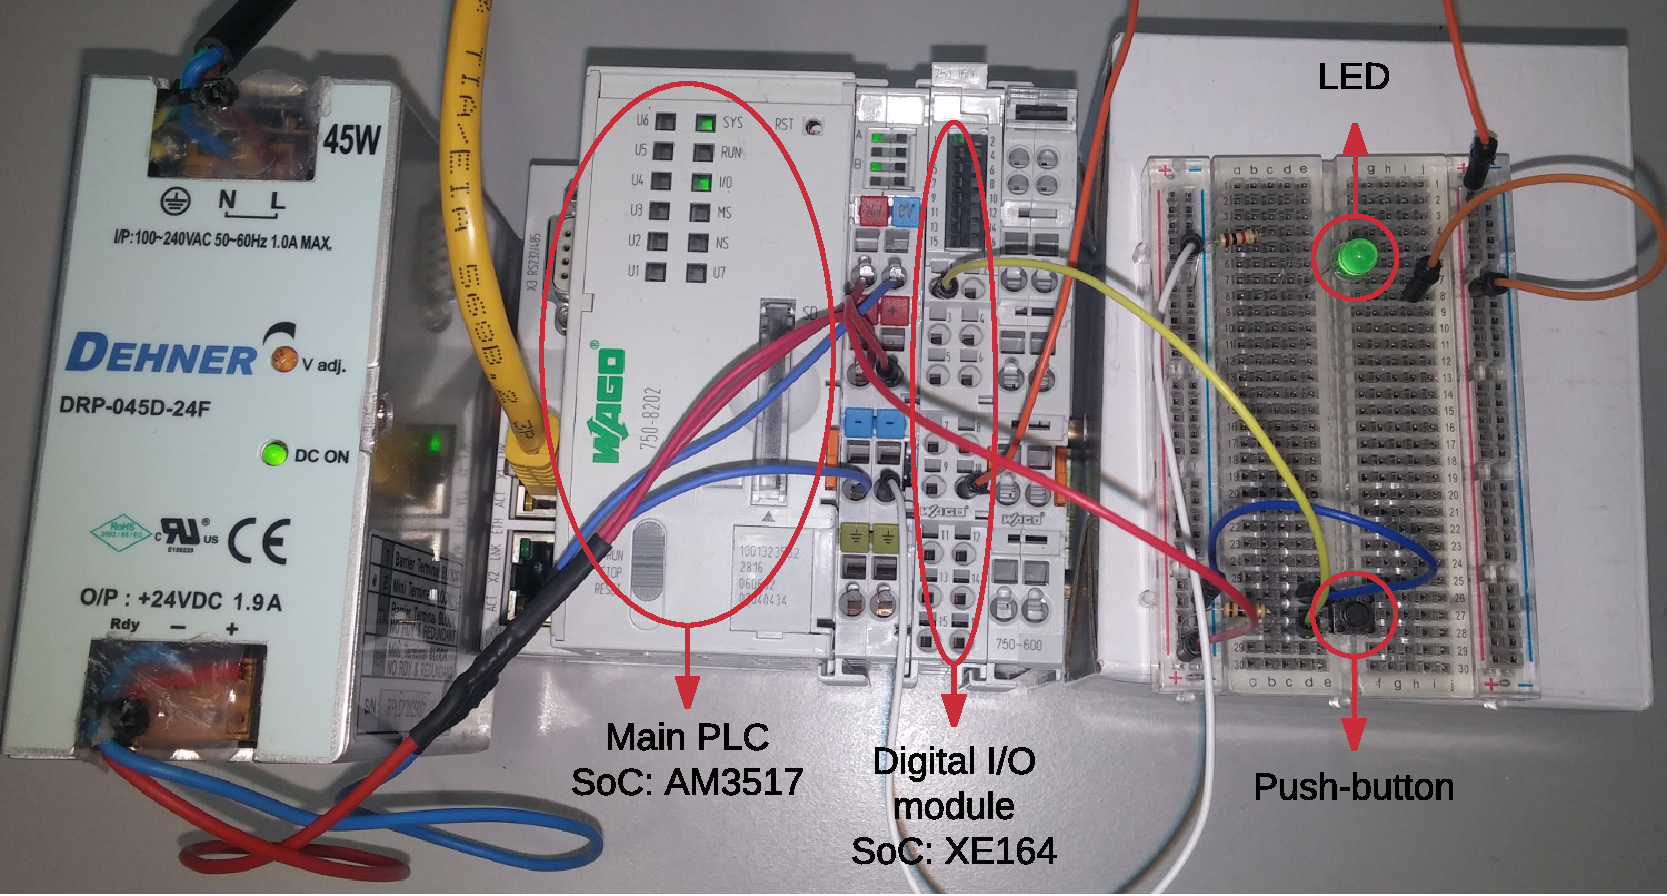
\includegraphics[width=0.8\textwidth]{res/plc_system}}
\caption{Wago PLC system used for experiments \label{fig:plc_system}}
\end{figure}

The PLC runtime environment is the \emph{e!RUNTIME} provided by Wago, which is always based on CODESYS. From the Wago \emph{e!COCKPIT} engineering software,
we programmed a simple logic which toggles the value of the LED every $\SI{500}{ms}$ only when the button is not pressed (high input). If the button is pressed,
the LED is turned off until the button is released. The logic, in \emph{Structured Text} (ST) language, is shown in \myfig{fig:plc_logic}.
It assumes a scan cycle of $\SI{10}{ms}$, and uses a software counter to achieve the timing of $\SI{500}{ms}$. The picture also shows the mapping between the variables
and the I/O pins of the external module. Differently from the Raspberry Pi system behaviour, here the outputs are updated on every scan cycle, even if the value has not been changed
during the last $\SI{10}{ms}$.
Given this system, we started the analysis of the PLC runtime to better understand the overall architecture, already reported in \mysec{sec:plc_arch}, and the Wago implementation.

\begin{figure}[h]
\centerline{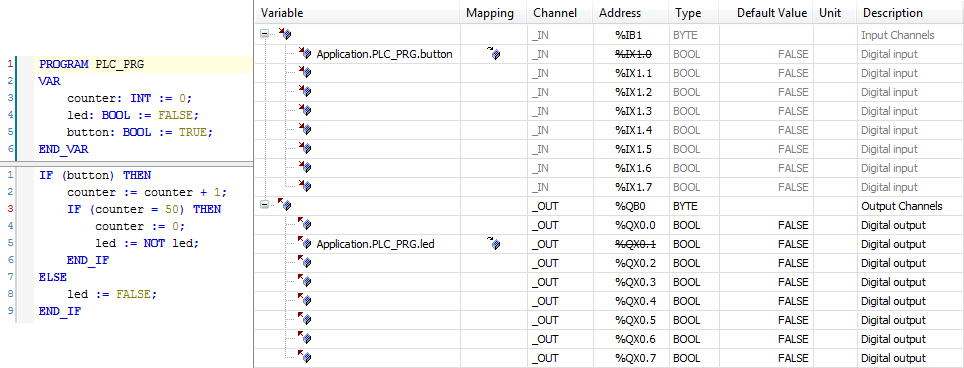
\includegraphics[width=\textwidth]{res/plc_logic}}
\caption{PLC logic loaded into Wago PLC \label{fig:plc_logic}}
\end{figure}


\subsubsection{PLC e!RUNTIME analysis}

For our research we used the following materials and tools:
\begin{itemize}
	\item \itemname{Board Support Package} (BSP) provided to us by Wago \cite{wago_linux}, which allows to build and configure a complete disk image
	of the system running inside the PLC. It essentially consists of: the kernel source code with all the patches applied by Wago, the libraries and
	the applications used into the system. For most of the Wago libraries, only the binary code is provided.
	\item \itemname{AM35x manual}: the Technical Reference Manual of AM35x processor, from \cite{am35x}.
	\item \itemname{strace} tool \cite{strace}, useful to analyse the behaviour of the PLC runtime, in particular the system calls used for accessing the I/O.
	\item \itemname{kprobes} kernel feature \cite{kprobes}, used to intercept function calls related to the I/O from kernel space.
\end{itemize}

We report the findings of our analysis as follows. With reference to the architecture described in \mysec{sec:plc_arch}, we discovered that the Wago implementation
uses a communication bus between PLC and I/O named \emph{KBUS}. It is implemented as a kernel driver, whose code is available as kernel patches included into the BSP.
The KBUS is basically a serial BUS built upon the Serial Peripheral Interface (SPI) protocol, used together with Direct Memory Access (DMA) to perform faster transfers.
From strace, we found that the PLC runtime uses the driver through \verb|ioctl| calls to send and receive inputs and outputs at each scan cycle, as reported below.
\begin{Verbatim}[fontsize=\small]
	[...]
	04:10:01.545185 clock_gettime(CLOCK_MONOTONIC, {122, 590121662}) = 0
	04:10:01.545831 clock_gettime(CLOCK_REALTIME, {1335924601, 545923773}) = 0
	04:10:01.546293 ioctl(11, _IOC(_IOC_WRITE, 0x4b, 0x01, 0x18), 0xb54a47d0) = 4
	04:10:01.549585 clock_gettime(CLOCK_REALTIME, {1335924601, 549739477}) = 0
	04:10:01.550047 clock_gettime(CLOCK_MONOTONIC, {122, 595045151}) = 0
	04:10:01.550508 nanosleep({0, 3785000}, NULL) = 0
	[...]
\end{Verbatim}
The code shows one PLC scan cycle, which is basically made of an \verb|ioctl| call, plus the corresponding calls needed to achieve the timing
of \SI{10}{ms} (\verb|clock_gettime| and \verb|nanosleep| functions).
Each \verb|ioctl| call from user space is directed to the internal \verb|kbus_ioctl| function of the KBUS driver.
\begin{figure}[h]
\centerline{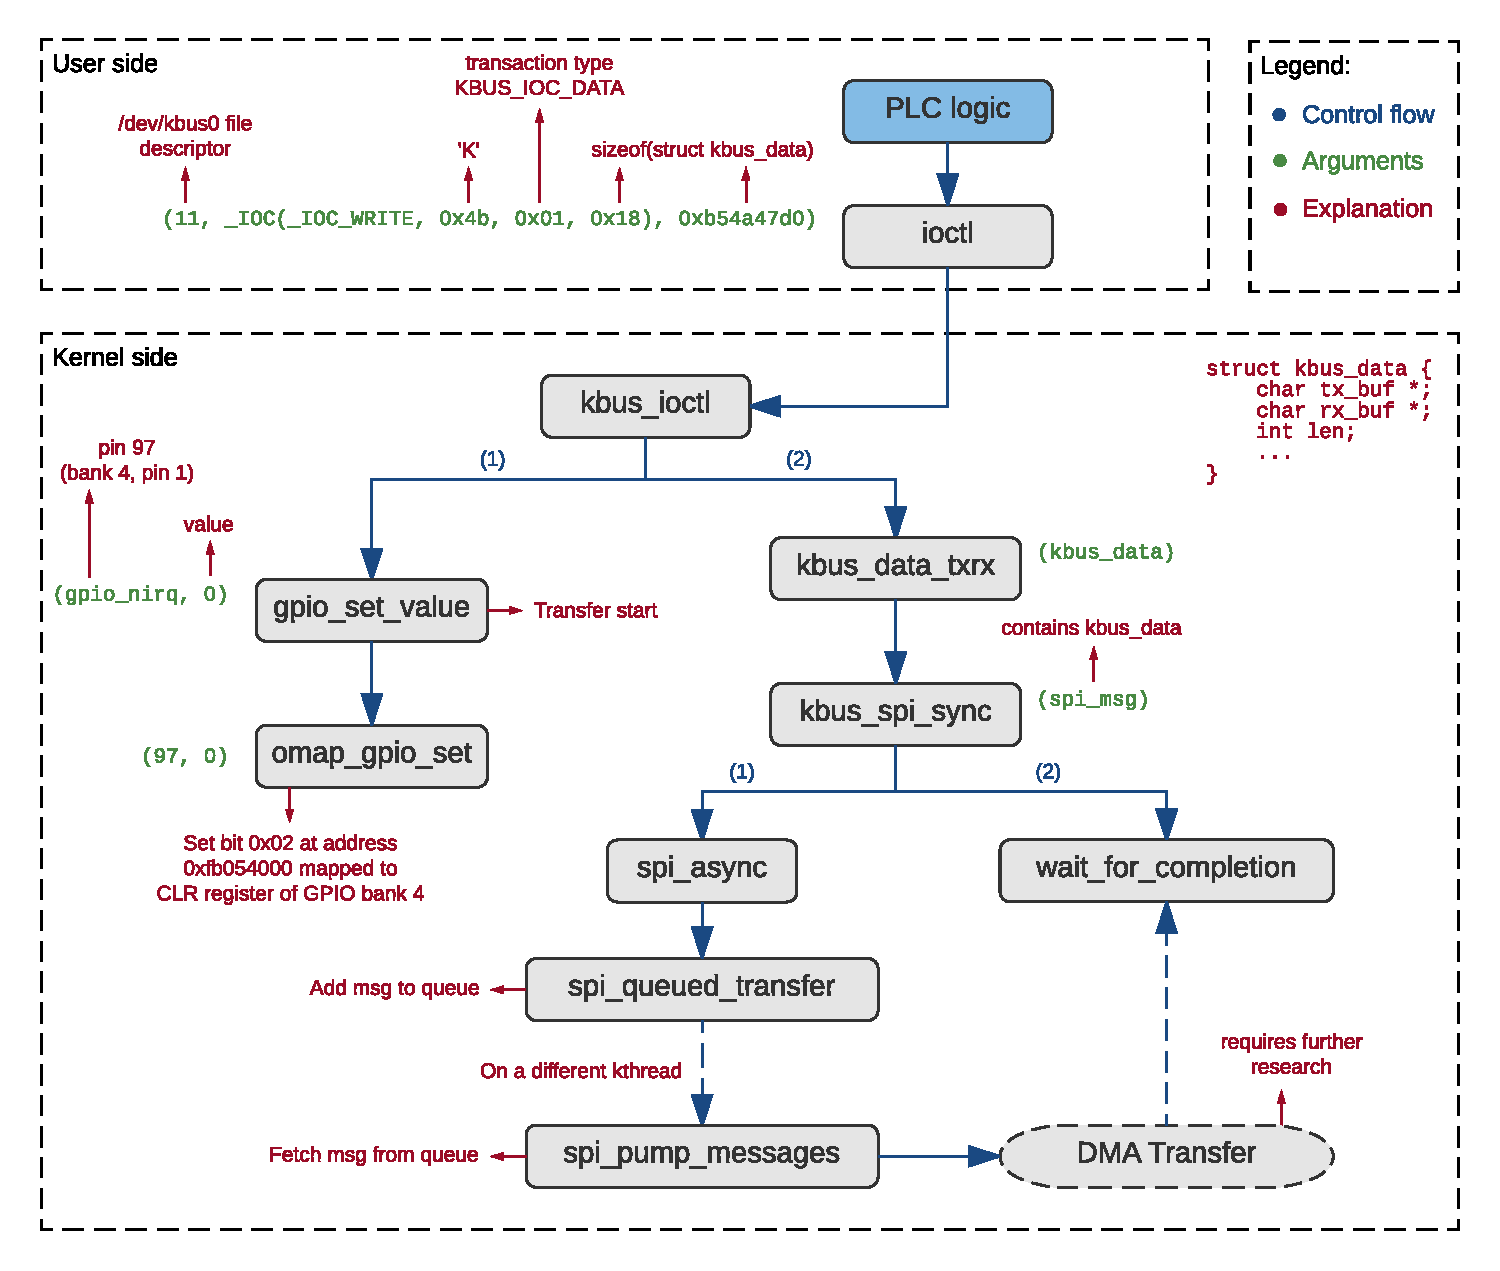
\includegraphics[width=\textwidth]{res/plc_io}}
\caption{PLC I/O operations executed for each scan cycle \label{fig:plc_io}}
\end{figure}
The operations performed at each scan cycle are outlined in the scheme of \myfig{fig:plc_io}, which shows the results of our reverse engineering analysis on Wago PLC e!RUNTIME.
From a quick look at the chart, we immediately deduce that the complexity is much bigger with respect to the CODESYS runtime for Raspberry Pi.
The important difference between CODESYS and e!RUNTIME is that the former performs I/O by directly mapping physical addresses and reading from (or writing to) I/O pins,
while the latter has to transfer data to the external I/O module. Thus, e!RUNTIME uses its I/O pins to communicate with I/O modules, by means of the KBUS driver interface.
KBUS is an abstraction layer built upon different lower-level drivers: basically GPIO, SPI and DMA.
The main operation of the kbus driver is managed through the \verb|kbus_ioctl| call. The first argument ($11$) is the file descriptor number related to the \verb|/dev/kbus0| file,
which allows the kernel to forward the request to the KBUS driver. The second argument contains different information used by the driver to select the specific sub-function.
In our case, the request is for a data transfer, and the third argument (\verb|0xb54a47d0|) is a pointer to a \verb|struct kbus_data|.
The data structure contains, among other members: a pointer to a transmit buffer (\verb|tx_buf|), a pointer to a receive buffer (\verb|rx_buf|) and a buffer length.
Since \verb|tx_buf| and \verb|rx_buf| are actually pointing to the same buffer used for both directions, only one length is required.
In our configuration, with the digital I/O module alone, the buffer contains at least $2$ bytes: one for input pins and one for output pins ($8$ bits each).
Thus, every \verb|ioctl| call serves both as read and write operation. On each call, the input part of the buffer is filled in by the KBUS driver,
while the output related to the previous scan cycle is written to the bus. From the new input obtained, the logic computes new output values,
waits for the necessary time, and calls \verb|ioctl| again with the updated buffer.
We report below the output of one of our kprobes to show the actual content of the buffer during a call to \verb|ioctl|:
\begin{Verbatim}[fontsize=\small]
	ioctl: len = 2, bytes = [0x40, 0x00]
\end{Verbatim}
The first byte indicates that the PLC logic is sending a $1$ to the second output pin (\verb|0x40|), to turn the LED on.
The second byte represents the input value related to the previous scan cycle, which will be overwritten by the KBUS driver during the current call.
In the above case, \verb|0x00| means that all the digital input lines were low.

Each I/O operation begins with a call to \verb|gpio_set_value|, which writes on a GPIO pin, indicating to the I/O module that a transfer is starting.
The pin used for this purpose is the GPIO pin $97$, \ie pin $1$ of GPIO bank $4$ (each bank controls $32$ pins). The value written into the pin is $0$,
since the signal is active low. Afterwards, the data buffer is encapsulated into an SPI message, starting an SPI transfer.
The SPI interface leverages four pins of the AM3517 SoC, two for data input and output (MOSI: Master Output Slave Input, and MISO: Master Input Slave Output),
one for synchronisation (SCL: Serial CLock) and one for chip select (SS: Slave Select).
The PLC SoC is the SPI master, and, according to our actual configuration, the digital I/O module is the only SPI slave available.
The transfer is delegated to the DMA controller, while the current thread, which corresponds to the PLC runtime thread,
goes to sleep into a wait condition (\verb|wait_for_completion|). Each DMA transfer uses an interrupt to signal when it has completed, or if some error occurred.
Further analysis is required to understand the behaviour of a DMA transfer and its corresponding IRQ handler, but that goes beyond the purpose of this master thesis.
Our best guess is that the DMA handler resets the initial GPIO pin and wakes up the PLC runtime thread.

Another interesting feature of the KBUS driver is that it exposes a \verb|write| operation to the user, through which it is possible to enable/disable the above interrupt.
The e!RUNTIME makes use of this system call to disable the interrupt while a new logic gets uploaded into the PLC, and then re-enables it before starting the logic.
If a new logic comes, together with a new I/O configuration, the interrupt gets disabled because the runtime needs to reprogram the I/O module
and the KBUS interface according to the new requirements. This behaviour gives us a hint to build another type of attack.
Our findings about possible attacks are described in the next section.


\subsubsection{PLC attack}

One of the first attack attempts we made was hooking the \verb|kbus_ioctl| function and tampering the values
inside the buffer. The effect was more powerful as the one achieved by Pin Control Attack, because we were able to control both inputs and outputs.
Anyway, this approach required function hooking, which is forbidden by our threat model (\mysec{sec:threat_model}).
A second attempt was multiplexing the SPI data pins to GPIO, to prevent the SPI controller to write to its I/O pins.
This condition, unfortunately, led to an indefinite wait of e!RUNTIME, noticeable by the operator running the e!COCKPIT software.
However, a better understanding of the SPI hardware protocol may allow the attacker to send fake data to the I/O module,
through a technique known as \emph{GPIO bit bang}. The bit banging technique consists of emulating in software all the operations made by
a hardware controller (\eg SPI) on I/O pins.

After having a good knowledge of the KBUS driver, we finally crafted three different attacks able to break the I/O communication without \emph{e!RUNTIME}
noticing anything and without hooking any function. The first two attacks are about Pin Configuration and Pin Multiplexing.
From the previous analysis, we know that the pin 97, multiplexed as GPIO and configured as output, is used by KBUS to send the \emph{transfer start} signal.
If we either multiplex or configure the pin in a different way, we are able to prevent e!RUNTIME from reading and writing values to the I/O.
This implementation demonstrates that I/O attack is perfectly applicable to real PLCs, even though it is still less powerful with respect to the
original version described in \mysec{sec:attack_pi}. In fact, our version enables the attacker to perform only one of the operations defined for Pin Control Attack:
disabling the output. Actually, since read and write are performed within the context of the same SPI transfer, also the input gets disabled at the same time.
However, this is irrelevant because the PLC logic cannot write to output in any case, independently from the input.
As discussed before, whether this operation may allow the attacker to alter the physical process, or not, is highly variable case by case.
For instance, in our target system, we proved that by repeating the attack every $\SI{50}{ms}$ with a trivial script, we were able to modify the logic behaviour:
the LED output started blinking every $\SI{50}{ms}$ instead of the original $\SI{500}{ms}$.
Furthermore, we found another interesting attack vector, which leverages the interrupt line used by the DMA controller and the \verb|write| interface provided by the KBUS driver.
Our experiments show that if this interrupt is masked while the PLC logic is running, the system is not able to read/write the I/O,
thus obtaining again the same effect as the previous implementation. Although it is still very simple, this kind of attack, which we can call \emph{IRQ Configuration Attack},
has some similarities with Pin Control Attack, such as the stealthiness and the hardware-level target.
The PLC runtime is not able to notice our attacks, no failures or errors are reported and no function hooks are required.
For both attack versions, the CPU overhead depends on the actual implementation, since the attacker can decide at which frequency disabling/enabling the I/O.
Generally speaking, the overhead is very low, because only one operation is needed to do/undo the attack, respectively, which is typically translated into two or three
processor instructions.

As discussed above, we believe that more sophisticated attacks are possible, since the basic hardware concepts described in \mysec{sec:embed_arch}
are still valid for a real PLC. The only difference is that, in this particular case, I/O pins are used as part of more complex protocols (SPI, DMA, etc.) and
they are multiplexed to the corresponding controllers inside the SoC. Therefore, to understand how each pin is used and to obtain more elaborated attacks
(\eg faking data via GPIO bit bang), further research effort is required.

To conclude our PLC analysis, we briefly describe the implementation of our attacks on Wago PLC.
Pin Configuration and Pin Multiplexing attacks are basically the same as for Raspberry Pi system. They can be executed in both kernel and user variants,
requiring the corresponding privilege level as discussed in \mysec{sec:attack_pi}.
One important difference here is that e!RUNTIME does not have its own mapped virtual addresses in user space, because the I/O is managed in kernel space
by the KBUS driver. Thus, we distinguish two cases:
\begin{itemize}
	\item \itemname{kernel-side attack}: the attacker can either remap the I/O physical addresses taken from the AM3517 manual \cite{am35x},
	or re-use the addresses already mapped by the pin control subsystem;
	\item \itemname{user-side attack}: the attacker can only request a new mapping to the kernel, because no other available mappings exist in user space.
\end{itemize}
Re-using already mapped addresses is theoretically feasible, because the control registers are actually mapped into the kernel, as reported by the output below.
\begin{Verbatim}[fontsize=\small]
	root@PFC200-4106BA:~ cat /proc/iomem 
	[...]
	48002030-48002267 : pinctrl-single
	48002a00-48002a5b : pinctrl-single
	[...]
\end{Verbatim}
However, the attacker needs to know the kernel virtual addresses (\eg by looking at page tables) in order to have access to the mapped registers.

Finally, for our IRQ configuration attack, we implemented it in two different variants as well: kernel side and user side.


\paragraph{Kernel side}

This version requires root privileges, since it is designed as a loadable kernel module.
The module leverages the \verb|disable_irq| function provided by the Linux kernel, which requires the interrupt line number to disable.
Thus, the attacker needs to know the target system model, but no knowledge of the PLC logic nor of the I/O mapping is required, because the system uses the same
configuration independently from the current logic.
We found the interrupt line number by inserting a kernel probe for the \verb|disable_irq| function, and triggering the PLC runtime to disable the interrupts
while loading a new logic.


\paragraph{User side}

This version requires at least the same privilege level of the PLC runtime, who is able to enable/disable the interrupt with the following operations (from strace):
\begin{Verbatim}[fontsize=\small]
	[...]
	04:09:46.008222 open("/dev/kbus0", O_RDWR) = 11
	[...]
	04:09:46.009237 write(11, "\x01\x00\x00\x00", 4) = 0
	[...]
	04:09:46.070565 write(11, "\x00\x00\x00\x00", 4) = 0
	[...]
\end{Verbatim}
Writing a $1$ into the \verb|/dev/kbus0| file disables the interrupt, while a $0$ enables it. We can implement the attack by emulating these PLC runtime operations from user space.
The effect of this second variant is the same as the kernel module one, but it requires less privilege and it could be exploited through a
remote code execution vulnerability of the PLC runtime, which is again based on CODESYS \cite{abb-codesys,codesys-server}.
